\subsection{Brief}
\paragraph{definition}
Image processing is the process of applying some operations to an image to reach an enhanced image
that satisfies a certain goal depending on the application in hand.
for example if we need to make an application that detects edges within an image we use an image processing
technique that is capable of highlighting those edges and make them stand out.
the result image is not necessarily a beautiful one from the perspective of a human, but it has to highlight
the features of interest within the image that would be used for further processing.

\paragraph{impact}
Apart from the rule image processing plays in graphics enhancement to make image more visually appealing,
Image processing is very important tool that is used for the specially preparation for computer vision and Machine learning, image processing a key preprocessing step to be taken before start in any of the two fields.
the key difference between those two purposes is that when we want the image to be more visually appealing
our target is a human, a human is the one who should view that image in the end.
but when it comes to fields like computer vision or Machine Learning, the target is a computer that is programmed 
to act based on the content of input image.
for this computer to do that it must be able to clearly extract feature of interest from the image, 
in order to make use of the image, we must have 2 main tasks for image processing:
\begin{enumerate}
	\item Noise Removal: to remove the noise (like salt and pepper, or gauessian blur, ...etc) that we estimate to exist in the image so as to refine the features to be extracted from the image.
	
	\item Feature Extraction: to highlight and evaluate features of interest that exist in the image to be used
	as input data for computer vision or Machine learning algorithms e.g. neural networks.
\end{enumerate}
these two processes are the most common use cases for image processing, and we will go over them with more detail in next section.


%---------------------------------------------------------------------------------
%---------------------------------------------------------------------------------
%---------------------------------------------------------------------------------
\begin{comment}
\subsection{How important is image processing?}
\paragraph{}
The applications of image processing are many we will catch on some applications for noise removal and feature extraction.
\subsubsection{Noise removal}
\paragraph{}
this process is done to make features more clear to refine the quality of extracted features by removing different types of noise (see figure 1.1).\newline
\begin{figure}{l}
	\centering
	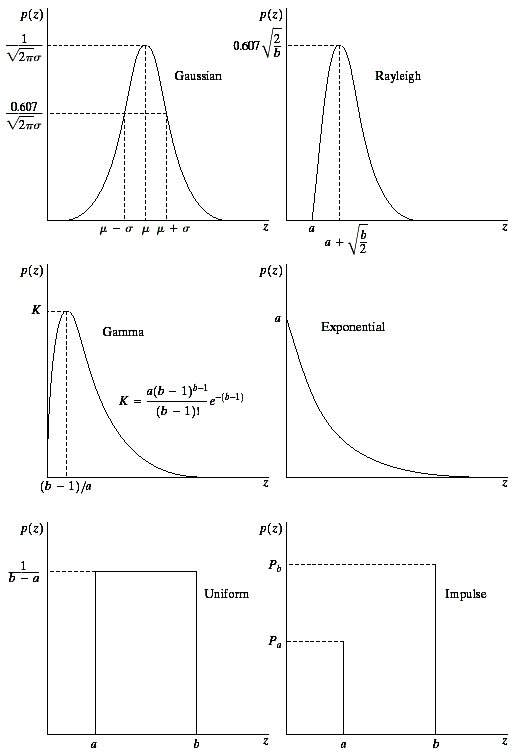
\includegraphics[width=0.5\textwidth]{CH1-introduction/sec2_image_processing/noise_types.png}
	\caption{examples for different types of noise}
\end{figure}
multiple filters exists to restore original image by removing noise as much as possible.
\begin{enumerate}
	\item Max filter: the output at one pixel is the \textbf{maximum} value of the pixels around it.
	\item Min filter: the output at one pixel is the \textbf{minimum} value of the pixels around it.
	\item Median filter: the output at one pixel is the \textbf{median} value of the pixels around it.
	\item Mean filter: the output at one pixel is the \textbf{mean} value of the pixels around it.
	\item Gauessian filter: it applies a matrix with values with gaussian distribution(highest weight in the center and weight decreases as we go away from the center) to the current window and the result is assigned to current pixel.
\end{enumerate}
these filters make use of the values of pixels around current pixel in order to detect abnormal changes within the image which is probably noise and based on the values of surrounding pixel a new value is assigned to current pixel which is estimated to be closest to the original value.\newline
Some other filter are used for enhancement can be sharpening filter and.

\subsubsection{Feature extraction}
this process is done to highlight features of interest in an image 
\end{comment}

%---------------------------------------------------------------------------------
%---------------------------------------------------------------------------------
%---------------------------------------------------------------------------------
\subsection{How is image processing important for our project}
The purposes of our project is to recognize the facial expression from face image, for this task multiple image 
processing techniques have been applied to the input image before extracting features like face landmarks and HOG from the image.

\subsubsection{Noise Removal}
since we don't expect the input image to be particularly corrupted we  use median filter to 
remove salt and pepper noise .
\begin{comment}
a gaussian filter was being used at as well but 
it was inefficient in terms of time so the median filter took its place without a problem.
\end{comment}
We also use sharpening filter to make face features more clear for the landmark extraction process.

\subsubsection{Feature Extraction}
unlike CNN (convolutional neural network) model which extracts the features it needs from the image directly, 
one of the approaches we took requires preprocessing to extract some features from input image
we needed two types of features in particular:
\begin{enumerate}
	\item HOG (Histogram of Oriented Gradients) : feature descriptor which means that it generalize the object in a way that the same object (in this case a person) produces as close as possible to the same feature descriptor when viewed under different conditions.
	\item Face Landmarks : those are points in the face that represent the face main features and we need those to estimate the emotion as well.
\end{enumerate}